\documentclass[11pt,letterpaper]{article}

% Use the custom AA279D template style
\usepackage{AA279D_template}
\usepackage{hyperref, gensymb, amsmath}

% User inputs: change as needed for each assignment
\newcommand{\workingDate}{\textsc{2018 $|$ April $|$ 16}}
\newcommand{\userName}{Yutao Liu}
\newcommand{\institution}{Stanford University}
\newcommand{\theTitle}{AA 279D}

\begin{document}
\title{279}
% Set up the title page
\begin{titlepage}
    \begin{center}
        \vspace*{1cm}
        
        \Huge
        \textbf{TanDEM-X/TerraSAR-X Constellation: Formation Flying in LEO}
        
        \vspace{0.5cm}
        \LARGE
        \ 
        
        \vspace{1.00cm}
        \textbf{\userName}
        \vspace{1.00cm}
        
        \vfill
        \begin{figure}[H]
		\centering 
		\includegraphics[width = 5.5in]{Figures/tt.jpg}
		\label{Figure: Title Graphic}
		\end{figure}
        \        
        
        \Large
        AA 279D - Spacecraft Formation-Flying and Rendezvous\\
        Stanford University\\
        
    \end{center}
\end{titlepage}

% Update the revision history with each assignment
\section*{Revision History}

\begin{table}[ht]
\centering
\caption{Summary of project revisions.}
\begin{tabular}{ll}
\toprule
\textbf{Rev} & \textbf{Changes} \\
\hline
PS1 & \tabitem Created document \\
    & \tabitem Added problem set 1 material  \\
\hline
PS2 & \tabitem Added problem set 2 material  \\
    & \tabitem Example revision statement 1  \\
    & \tabitem Example revision statement 2  \\
\hline
PS3 & \tabitem Added problem set 3 material  \\
\bottomrule
\end{tabular}
\label{table:revision history}

\end{table}

\newpage
\tableofcontents

\newpage
\section{Preliminary mission study}
\subsection{Mission description}
The TanDEM-X spacecraft launched on 21 June 2010 complements the existing TerraSAR-X satellite to form the first configurable SAR (Synthetic Aperture Radar) interferometer with baselines of a few hundred meters in space. The primary goal of the TanDEM-X (TerraSAR-X add-on for Digital Elevation Measurement) mission is to generate a global digital elevation model (DEM). 

The satellites will fly in formation and operate in parallel for three years to cover the entire surface of Earth. Together, the  identical spacecrafts orbit Earth in a polar dusk-dawn orbit with a 515 km altitude and an 11 day repeat period. Besides controlling the TerraSAR-X spacecraft to fly in a predefined tube of 250 m radius, regular control maneuvers will be exercised to maintain a specific formation geometry in each mission phase.\cite{montenbruck}

A schematic representation of the satellites as well as their operating conditions can be found below.
\begin{figure}[H]
	\centering
    \includegraphics[height=3in]{Figures/tandem.jpg}
    \caption{The TerraSAR-X and TanDEM-X satellites are nearly identical in construction.}
    \label{figure:Sats}
\end{figure}

\begin{table}[ht]
\centering
\caption{Satellite specifications}
\label{my-label}
\begin{tabular}{ll}
\toprule
Orbit altitude       & 514 km \\
Orbit inclination    & 97.4\degree   \\
Satellite mass       & 1330 kg \\
Satellite dimensions &                \\
Height               & 5 m       \\
Diameter             & 2.4 m    \\
\bottomrule
\end{tabular}
\end{table}

The up-to-date orbital elements of the constellation could be retrieved from \href{www.heavens-above.com}{heavens-above.com}:
\begin{table}[ht]
\centering
\caption{Current orbital elements}
\label{my-label}
\begin{tabular}{lll}
\toprule
\textbf{Orbital Element	}		   & \textbf{TerraSAR-X}   & \textbf{TanDEM-X}      \\
\hline
Epoch (UTC):                       & 16 April 2018 04:07:14 & 16 April 2018 07:16:58 \\ 
Eccentricity:                      & 0.0002035              &.0002293                \\ 
Inclination:                       & 97.4464\degree         & 97.4452\degree \\
Perigee height:                    & 507 km                 & 507 km\\
Apogee height:                     & 510 km                 & 510 km\\
Right ascension of ascending node: & 114.6359\degree        & 114.5018\degree \\
Argument of perigee:               & 72.8528\degree         & 77.4517\degree \\
Revolutions per day:               & 15.19142245            & 15.19144898 \\
Mean anomaly at epoch:             & 344.5982\degree        & 339.8946\degree \\
Orbit number at epoch:             & 43363                  & 60087 \\
\bottomrule
\end{tabular}
\end{table}

\subsection{Mission Orbit Simulation}
The first step in the mission study would be to simulate the trajectory of TerraSAR-X, which was launched 15 June 2007, 02:14 UTC into a polar,  sun-synchronous dusk-dawn orbit at 514km altitude. This forms an ellipse of 6886.39 km semi-major axis and 0.0001445 eccentricity at an inclination of 97.44\degree.

\begin{figure}[H]
	\centering
    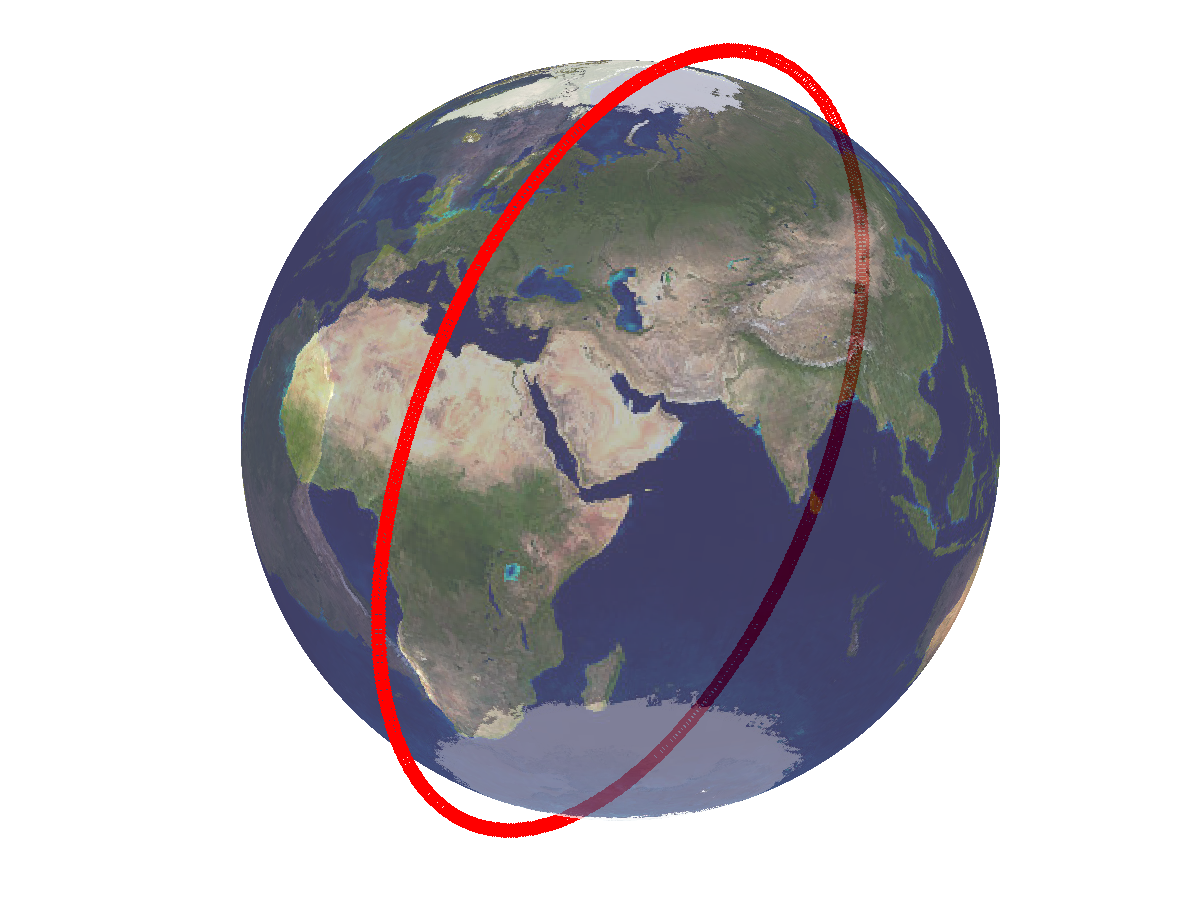
\includegraphics[height=3in]{Figures/Traj.eps}
    \caption{Osculating orbit of TerraSAR-X}
    \label{figure:traj}
\end{figure}
\subsubsection{Effects of $J_2$ perturbation}
% Equation \ref{Equation: golden rule} is demonstrating the use of custom commands embedded in the .sty sheet which can simplify your main LaTeX document.
% \begin{align}
% 	\VEL{N}{A_0} &= \DIFF{N}{ \POS{N_0}{A_0} } = \VEL{R}{A_0} + \OMEGA{N}{R} \times \POS{N_0}{A_0}
% 	\label{Equation: golden rule}
% \end{align}
% where $\VEL{N}{A_0}$ is the velocity of point $A_0$ in reference frame $\FRAME{N}$, $\VEL{R}{A_0}$ is the velocity of $A_0$ in reference frame $\FRAME{R}$, $\OMEGA{N}{R}$ is the angular velocity of $\FRAME{R}$ in $\FRAME{N}$, and $\POS{N_0}{A_0}$ is the position vector from point $N_0$ (which is fixed in $\FRAME{N}$) to $A_0$.\\

% Absolute value: $\abs{-5} = 5$.\\
% Vector norm: $\norm{\vec{r}} = \sqrt{r_X^2 + r_Y^2 + r_Z^2}$\\



\section{Relative motion study}

\begin{figure}[H]
	\centering
    \includegraphics[height=3in]{Figures/monobi.jpeg}
    \caption{Concept of TanDEM-X InSAR observations in bistatic (left) and monostatic (right) modes}
    \label{figure:modes}
\end{figure}

\begin{figure}[H]
	\centering
    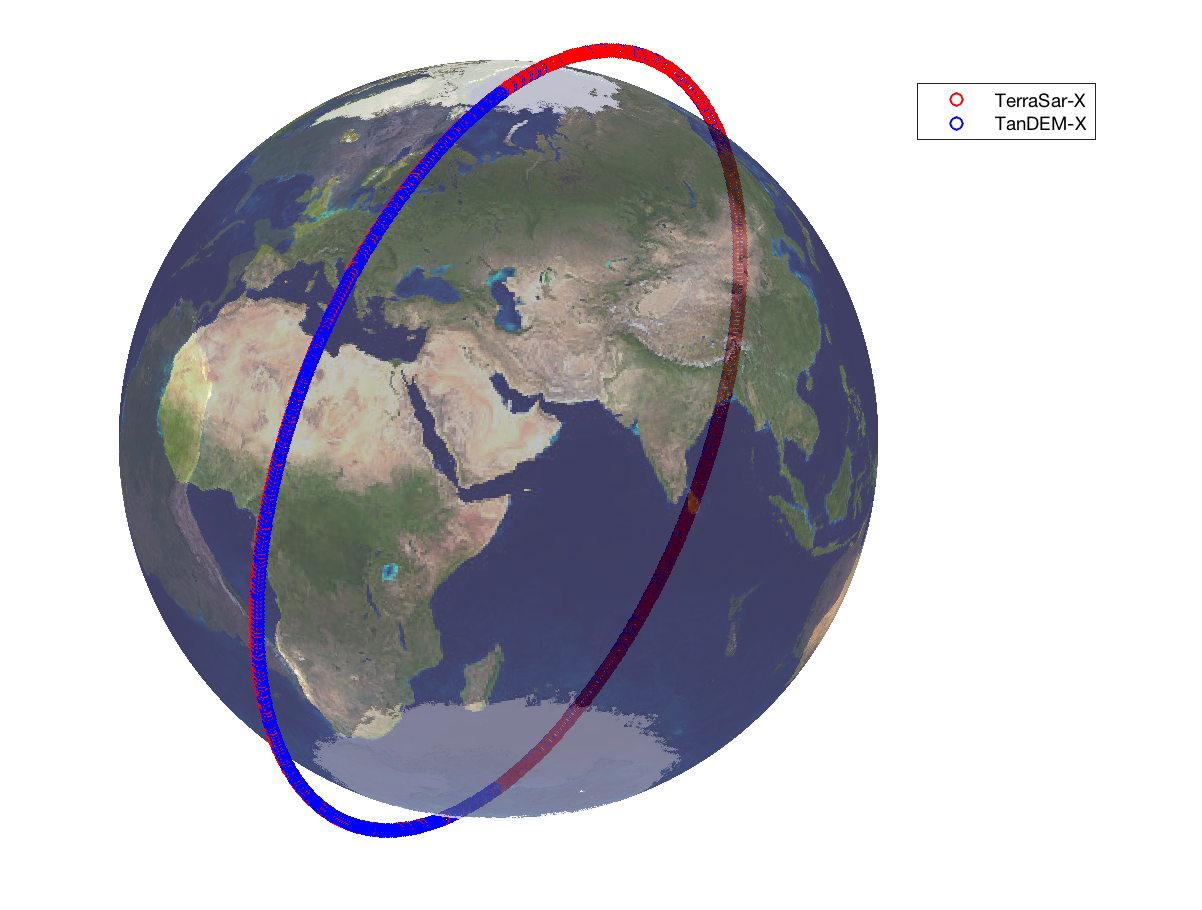
\includegraphics[height=3in]{Figures/Traj2.eps}
    \caption{Simulation of TerraSAR-X and TanDEM-X trajectories}
    \label{figure:traj}
\end{figure}

\section{Linear Relative Motion}
\section{perturbed J2 relative orbit motion in close near-circular  orbits  using  analytic  solutions  and  numerical  integration}
\section{Control Law Requirements}
What are the significant operational modes of your formation?  Some examples may include safe-keeping mode, scientific observation mode, and rendezvous/docking mode,though the needs of your mission may vary.  Be sure to define at least 2-3 modes.

How are these modes defined?  Think about the absolute and relative motions of your spacecraft.  You might use sets of absolute or relative orbit elements to characterize each mode, for example.

When  operating  within  these  modes  (i.e.   formation  keeping),  what  sorts  of  control requirements may your formation be subjected to?  You should consider parameterslike allowable separations, necessary precision of knowledge and actuation, limitations on burns, etc.

When switching between modes (i.e.  reconfiguration), what kinds of control requirements are present?  Some examples include time to reconfigure or any safety concerns.

\section{Control Law Implementation}

\section{Navigation System Design}
What  relative  state  representation  will  you  estimate  with  your  filter?   Examples  we have seen in class include the Cartesian relative state, orbit element differences, and quasi-nonsingular relative orbit elements.

What dynamics model will you use to perform the EKF state prediction?  Will you per-form the prediction with a closed-form linear/nonlinear propagator or with a numerical integration scheme?

What is the associated linearized dynamics model you will use to perform the EKF covariance update?  Provide the state transition matrixΦand control input matrixB.

What sensors are available on-board your spacecraft, and what kinds of measurements do they provide (e.g.  GNSS, radio frequency, optical, etc.)?•What is the nonlinear model which relates the state to the sensor measurements?

What is the associated sensitivity matrix H which you will use to perform the EKF update step?

\section{Navigation System Implementation}
Generate ground truth signals using a clearly-described formation propagator.•Consider two types of measurements:1.  Corrupt  the  ground  truth  state  of  interest  with  some  Gaussian  noise  and  feedthis to the EKF (i.e.yt=Ixt+vt, wherevtis zero-mean white noise).  Use thissimplified set of measurements to validate your filter’s base performance.2.  Generate representative measurements according to your mission’s sensors usingthe nonlinear measurement model from Part 1.In  both  of  the  above  cases,  be  sure  to  use  apply  reasonable  levels  of  noise  for  yourmeasurements based on the accuracy of your sensors.Note that you can generate noise as a zero-mean Gaussian random vector with prese-lected standard deviation in MATLAB assqrtm(sigma)*randn(n, 1), wheresigmais a covariance matrix, andnis your desired vector size.•Set an initial estimate and covariance,x0andP0.  The estimate should be close to,but not exactly equal to the true initial state.  The covariance can be set to a diagonalmatrix, with elements equal to the variance of your state parameters.•Define the process and measurement noise covariances,QandR, which represent theuncertainty in the dynamics and measurement models, respectively.  You may wish todefineQsimilar toP0, but much smaller.  MeanwhileRmay be a diagonal matriceswith elements equal to the variance of each measurement.•Combine all of the previous parameters and mechanize your extended Kalman filter.Recall the steps involved in a single iteration of the EKF:1.  Predict the evolution of the state and covariance with your dynamics model andstate transition matrix.2.  Generate a pre-fit residual by comparing the expected measurement against thetrue measurement.3.  Update the prediction with the EKF measurement update step.4.  Generate  a  post-fit  residual  by  comparing  the  updated  expected  measurementagainst the true measurement.•Illustrate the performance of the filter by plotting the following parameters: true, mea-sured, and estimated states, estimation error (difference between true and estimatedstates), standard deviation of the estimate, and pre-fit and post-fit residuals.

\section{Filter Integration}
Select at least one control law you wish to analyze from Problem Set 6.(b)  Alter the control law state input by corrupting the ground truth with some represen-tative noise.  The bias and covariance of this noise should match the expected behaviorof your estimator, similar to the process you used to generate your first set of measure-ments in Problem Set 7, Problem 2.  How does your controller perform?  What are themain differences compared to the original implementation?(c)  Now use the extended Kalman filter from Problem Set 7 to feed the control law itsstate input.  You should send the ground truth through your true sensor model, thenfeed this to the filter before passing the estimated state to the controller.  Note thatyou must now account for the introduction of control inputs in the prediction step ofyour EKF. How does the controller perform?For both of the simulations in parts (b) and (c), you should provide comprehensive perfor-mance metrics.  These include parameters like the time to convergence (i.e.  when the errorfalls below a certain threshold), control tracking error/navigation error and their statisticsat  steady  state,  comparison  of  pre-  and  post-fit  residuals,  control  input  history,  ∆Vcon-sumption, etc.  Be sure to discuss how performance compares with your expectations.



% % \documentclass[11pt,letterpaper]{article}

% % Use the custom AA279D template style
% \usepackage{AA279D_template}
% \usepackage{hyperref, gensymb, amsmath}
% \begin{document}

$$^\mathbb{I}{\delta\mathbf{v}_L} = ^\mathbb{I}{\mathbf{R}}^\mathcal{L}$$
orbit design usually done in mean space $\langle\cdot\rangle$

osculating oe as a transformation from mean
$\textbf{\oe}(\langle\textbf{\oe}\rangle)$

use Newton-Raphson to compute $\langle\Delta\textbf{\oe}\rangle$ iterative update until error condition

$$\ddot{\mathbf{\rho}} = 
\mathbf{f}
(\mathbf{\rho}, \dot{\mathbf{\rho}}, \mathbf{r}_0, \dot{\mathbf{r}}_0, \mathbf{\theta}_0, \dot{\mathbf{\theta}}_0,)
$$
when $e_0=0$ this becomes $\ddot{\mathbf{\rho}} = 
\mathbf{g}(\mathbf{\rho}, \dot{\mathbf{\rho}}, \mathbf{\theta}_0,)$

when will the deputy appear stationary to the chief?

\[
	\begin{cases}
    	(x+a_0)^2 + y^2 = a_0^2\\z=0
    \end{cases}
\]

when $\rho/r_0 <<1$ the HOTs drop out to yield a set of linear ODEs
\[
	\begin{cases}
    \begin{aligned}
    	&\ddot{x}-2n_0\dot{y} &-3n^3x &=0\\
        &\ddot{y}+2n_0\dot{x} &       &=0\\
        &\ddot{z}&+n_0^2z             &=0
    \end{aligned}
    \end{cases}
\]

can you replace mean motion of chief with deputy? no longer second order

FF in LEO of small separations can be designed with HCW equations

% \end{document}

%%%%%%%%%%%%%%%%%%%%%%%%%%%%%%%%%%%%%
% References
%%%%%%%%%%%%%%%%%%%%%%%%%%%%%%%%%%%%%
\newpage
\begin{thebibliography}{9}
\bibitem{alfriend}K. Alfriend, S. Vadali, P. Gurfil, J. How, and L. Breger, \textit{Spacecraft Formation Flying: Dynamics, Control, and Navigation}. Elsevier Astrodynamics Series, 2010. 

% https://onlinelibrary.wiley.com/doi/epdf/10.1002/j.2161-4296.2011.tb02587.x
\bibitem{montenbruck}O. Montenbruck, M. Wermuth, and R. Kahle,
\textit{GPS Based Relative Navigation for the TanDEM-X Mission - First Flight Results}. DLR/GSOC, September 2010.

% http://elib.dlr.de/63481/1/Damico_PhD_01022010.pdf
\bibitem{damico}S. D'Amico, \textit{Autonomous Formation Flying
in Low Earth Orbit}. PhD Thesis. TU Delft, 2010.

% 

\end{thebibliography}
\addcontentsline{toc}{section}{References}

\end{document}